\chapter{The Effects of Na$_{2}$O and SiO$_{2}$ on Liquid Phase Sintering of Bayer Al$_{2}$O$_{3}$}

\section{Introduction}
Al$_{2}$O$_{3}$ is arguably the most extensively used and researched ceramic material because it is used in many large volume applications such as high temperature refractories, technical ceramics, high voltage insulators, and functional fillers. The majority of Al$_{2}$O$_{3}$ applications use synthetic or specialty aluminas derived from Bayer feedstocks, such as aluminum trihydrate (Al(OH)$_{3}$), smelter grade Al$_{2}$O$_{3}$ and others. Bayer process aluminas are typically 99.0 - 99.9\% pure and contain Na$_{2}$O, CaO, Fe$_{2}$O$_{3}$, and SiO$_{2}$ impurities that originate from the bauxite ore and/or Bayer process reagents (e.g., NaOH). The vast majority of research on the sintering of Al$_{2}$O$_{3}$, however, focuses on ultra-high purity (≥ 99.99\%) aluminas derived from specialty feedstocks, such as ammonium alum (NH$_{4}$Al(SO$_{4}$)$_{2}$$\cdot$12H$_{2}$O), boehmite ($\gamma$-AlOOH) and aluminum chloride (AlCl$_{3}$). While ultra-high purity aluminas provide the purest platform from which to conduct fundamental sintering research, that research does not usually explore the types and amounts of impurities typical of Bayer aluminas.  Commercial Bayer Al$_{2}$O$_{3}$ powders exist in a range of reactive grades that differ in the amount and types of these impurities. Therefore, the evaluation of specialty reactive aluminas, within the context of previous work on ultra-high purity aluminas, is a valuable contribution to industrial users and bridges fundamental sintering research with ultra-high purity aluminas.


\section{Experimental}

A chemically purified 0.4 $\mu$m median particle size Bayer process Al$_{2}$O$_{3}$ powder (Almatis, Inc., Leetsdale, PA, USA) with only 2 ppm MgO was used to study the sintering of near MgO-free Bayer Al$_{2}$O$_{3}$ (Figure \ref{Ch3-figure:Figure1}). The powder was chemically purified by the manufacturer so that impurity levels similar to commercial high purity Bayer process aluminas were obtained after doping with Na$_{2}$O and/or SiO$_{2}$. The physical and chemical characteristics of the as-received powder are shown in Table \ref*{Ch3-table:chembayer}. Chemical analysis of the as-received Al$_{2}$O$_{3}$ was performed by inductively coupled plasma (ICP) emission spectroscopy (iCap 6000, Thermo Fischer Scientific, Inc., Waltham, MA, USA) after Al$_{2}$O$_{3}$ samples were acid digested in a microwave digestion unit in a Teflon$^{TM}$ sample holder.  It should be noted that the as-received Bayer Al$_{2}$O$_{3}$ contained impurity levels of 90 ppm Fe$_{2}$O$_{3}$, 62 CaO, and 22 ppm TiO$_{2}$.  The Na${2}$O and SiO$_{2}$ reported after doping include the impurity concentrations in the as-received powder (29 ppm Na$_{2}$O and 103 ppm SiO$_{2}$). 

The Al$_{2}$O$_{3}$ powders were doped with up to 1000 ppm Na$_{2}$O using sodium acetate (NaC$_{2}$H$_{3}$O$_{2}$$\cdot$3H$_{2}$O, ACS grade, BDH, West Chester, PA, USA), based on the procedure reported by Louet et al. \cite{Louet2005}. The Al$_{2}$O$_{3}$ powders were dispersed in a solution of sodium acetate dissolved in de-ionized water. The suspension was stirred on a magnetic stir plate for 5 h at room temperature, and held at 80$^{\circ}$C for 24 h while stirring until the mixture was too viscous to stir, and then dried at 100$^{\circ}$C for 24 h. 

Samples were doped with up to 500 ppm SiO$_{2}$ by first dissolving tetraethyl orthosilicate (TEOS, Si(OC$_{2}$H$_{5}$)$_{4}$, 98\%, Aldrich Chemical Company, Inc., Milwaukee, WI, USA) in 200 proof ethanol with a few drops of de-ionized water to hydrolyze the TEOS and immediately mixed at room temperature for 5 h with either the as-received or Na$_{2}$O-doped Al$_{2}$O$_{3}$ powder. The mixture was subsequently stirred at 70$^{\circ}$C for an additional 12 h. The powder was then dried at 100$^{\circ}$C for 2 h, followed by crushing in a mortar and pestle, and sieving to -106 $\mu$m (US Standard 140 mesh).

Samples were prepared for sintering studies by uniaxially dry pressing the powders at 170 MPa and then cold isostatic pressing at 200 MPa (CIP, Autoclave Engineers, Erie, PA, USA) to obtain cylindrical samples (3.0-3.5 mm long by 12.7 mm diameter or 8.5-10 mm long by 6 mm diameter) with green densities of 59.0\% $\pm$ 0.5\% of theoretical density. To investigate the sintering process, dry pressed 8.5-10 mm long by 6 mm diameter cylinders were heated at 10$^{\circ}$C/min to 1525$^{\circ}$C in a thermomechanical analyzer (TMA, Linseis PT1600, Robbinsville, NJ, USA). The kinetics of sintering and grain growth were evaluated on 3.0-3.5 mm long by 12.7 mm diameter samples heated at 10$^{\circ}$C/min to 1200 $^{\circ}$C then 5$^{\circ}$C/min to 1525$^{\circ}$C followed by sintering at 1525$^{\circ}$C for up to 8 h. The density of three samples of each condition was measured by the Archimedes method according to ASTM standard B962-15 \cite{Standard2015} and the average density reported for each sintering time and temperature. For microstructure analysis, samples were first polished to a surface finish of 1 $\mu$m and then thermally etched in air at 1425$^{\circ}$C for 40 min. Average grain sizes were measured on SEM (ESEM, Quanta 200, FEI Company, Hillsboro, OR, USA) micrographs using a linear intercept method (ASTM Standard E112-96) \cite{Standard2013}.

\section{Results}

\subsection{Effects of Na$_{2}$O-doping}

The doping experiments were designed to uniformly distribute Na$-{2}$O and SiO$_{2}$ on the surfaces of the Al$_{2}$O$_{3}$ particles. Upon heating the dopant NaC$_{2}$H$_{3}$O$_{2}$$\cdot$3H$_{2}$O first dehydrates and then decomposes to form Na$_{2}$CO$_{3}$ above 385$^{\circ}$C \cite{Judd1974}. Using a video recorder, we observed that anhydrous sodium acetate melts and rapidly spreads on the surface of an Al$_{2}$O$_{3}$ substrate at $\sim$420$^{\circ}$C. Na$_{2}$CO$_{3}$ melts at 851$^{\circ}$C and subsequently decomposes to Na$_{2}$O \cite{Judd1974}. As a result of the rapid wetting of the Na$_{2}$O precursor on the Al$_{2}$O$_{3}$ substrate we conclude that Na$_{2}$O is uniformly distributed on the powder surface by the acetate doping process. 

Figure \ref{Ch3-figure:Figure2} shows the shrinkage behavior of Bayer Al$_{2}$O$_{3}$ doped with different Na$_{2}$O concentrations during heating to 1525$^{\circ}$C at 10$^{\circ}$C/min. The as-received Al$_{2}$O$_{3}$ (intrinsic impurities: 29 ppm Na$_{2}$O, 103 ppm SiO$_{2}$) begins to shrink at $\sim$1050 $^{\circ}$C, whereas shrinkage begins at 1100$^{\circ}$C for samples doped with 1029 ppm Na$_{2}$O. The difference in density at the beginning of densification continues throughout the heating cycle. However, above $\sim$1350$^{\circ}$C the densification rate of the Na$_{2}$O doped samples surpasses that of the as-received sample. Overall, the Na$_{2}$O-doped samples are 2.5\% less dense than the as-received Al$_{2}$O$_{3}$ after heating to 1525$^{\circ}$C.



\newpage
\begin{table}[H]
	\caption{Physical and chemical characteristics of the as-received Bayer Al2O3 powder used in this study.}
	\centering
	\begin{tabular}{ | c | c | }
		\hline
		 & \\
		\hline
		BET (m$^{2}$/g) & 7.4 \\
		\hline
		D$_{50}$ ($\mu$m) & 0.4 \\
		\hline
		D$_{90}$ ($\mu$m) & 1.5 \\
		\hline
		 & ICP (ppm) \\
		\hline
		Al$_{2}$O$_{3}$ & 99.96 \% \\
		\hline
		SiO$_{2}$ & 103 \\
		\hline
		Na$_{2}$O (total) & 29 \\
		\hline
		Fe$_{2}$O$_{3}$ & 90 \\
		\hline
		CaO & 62 \\
		\hline
		TiO$_{2}$ & 22 \\
		\hline
		MgO & 2 \\
		\hline
	\end{tabular}
	\label{Ch3-table:chembayer}
\end{table}
\clearpage
%%%

\newpage
\begin{table}[H]
	\caption{Calculated compositions and amounts of liquid in as-received, singly doped and co-doped samples at 1525$^{\circ}$C ($\alpha$ = $\alpha$-Al2O3, $\beta$ = $\beta$-Al2O3, L = liquid, M = mullite).}
	\centering
	\resizebox{\textwidth}{!}{\begin{tabular}{ | c | c | c | c | c | c | c | c | c | }
		\hline
		\multicolumn{2}{|l|}{Global dopant} & Global & Na$_{2}$O:SiO$_{2}$ & \multicolumn{3}{l|}{Composition} & Amount & Stable \\
		\multicolumn{2}{|l|}{concentration} & Na$_{2}$O:SiO$_{2}$ & ratio in & \multicolumn{3}{l|}{of liquid} & of liquid & phases \\
		\cline{1-2}
		ppm (wt.) & ppm (mol) & ratio & Liquid & \multicolumn{3}{l|}{(mol \%)} & (vol. \%) & \\
		\cline{5-7}
		Na$_{2}$O/SiO$_{2}$ & Na$_{2}$O/SiO$_{2}$ & & & Na$_{2}$O & SiO$_{2}$ & Al$_{2}$O$_{3}$ & & \\
		\hline
		As-received & & & & & & & & \\
		29/103 & 48/175 & 0.27 & 0.25 & 17.9 & 63.4 & 19.7 & 0.03\% & $\alpha$+L \\
		\hline
		154/103- & 253/175- & & & & & & & \\
		1029/103 & 1693/175 & 1.45-9.67 & 0.5 & 26.1 & 52.3 & 21.6 & 0.03\% & $\alpha$+L+$\beta$ \\
		\hline
		29/603 & 48/1023 & 0.05 & 0.25 & 16.3  & 65.3 & 18.4 & 0.03\% & $\alpha$+L+M \\
		\hline
		154/603 & 253/1023 & 0.25 & 0.25 & 16.3 & 65.3 & 18.4 & 0.16\% & $\alpha$+L \\
		\hline
		279/603 & 459/1023 & 0.45 & 0.45 & 24.5 & 54.6 & 20.8 & 0.19\% & $\alpha$+L \\
		\hline
		529/603 & 870/1023 & 0.85 & 0.5 & 26.1 & 52.3 & 21.6 & 0.22\% & $\alpha$+L+$\beta$\\
		\hline
		1029/603 & 1693/1023 & 1.65 & 0.5 & 26.1 & 52.3 & 21.6 & 0.22\% & $\alpha$+L+$\beta$ \\
		\hline
	\end{tabular}}
	\label{Ch3-table:liquidbayer}
\end{table}
\clearpage
%%%

\newpage
%%%
\begin{figure}[H]
	\centering
	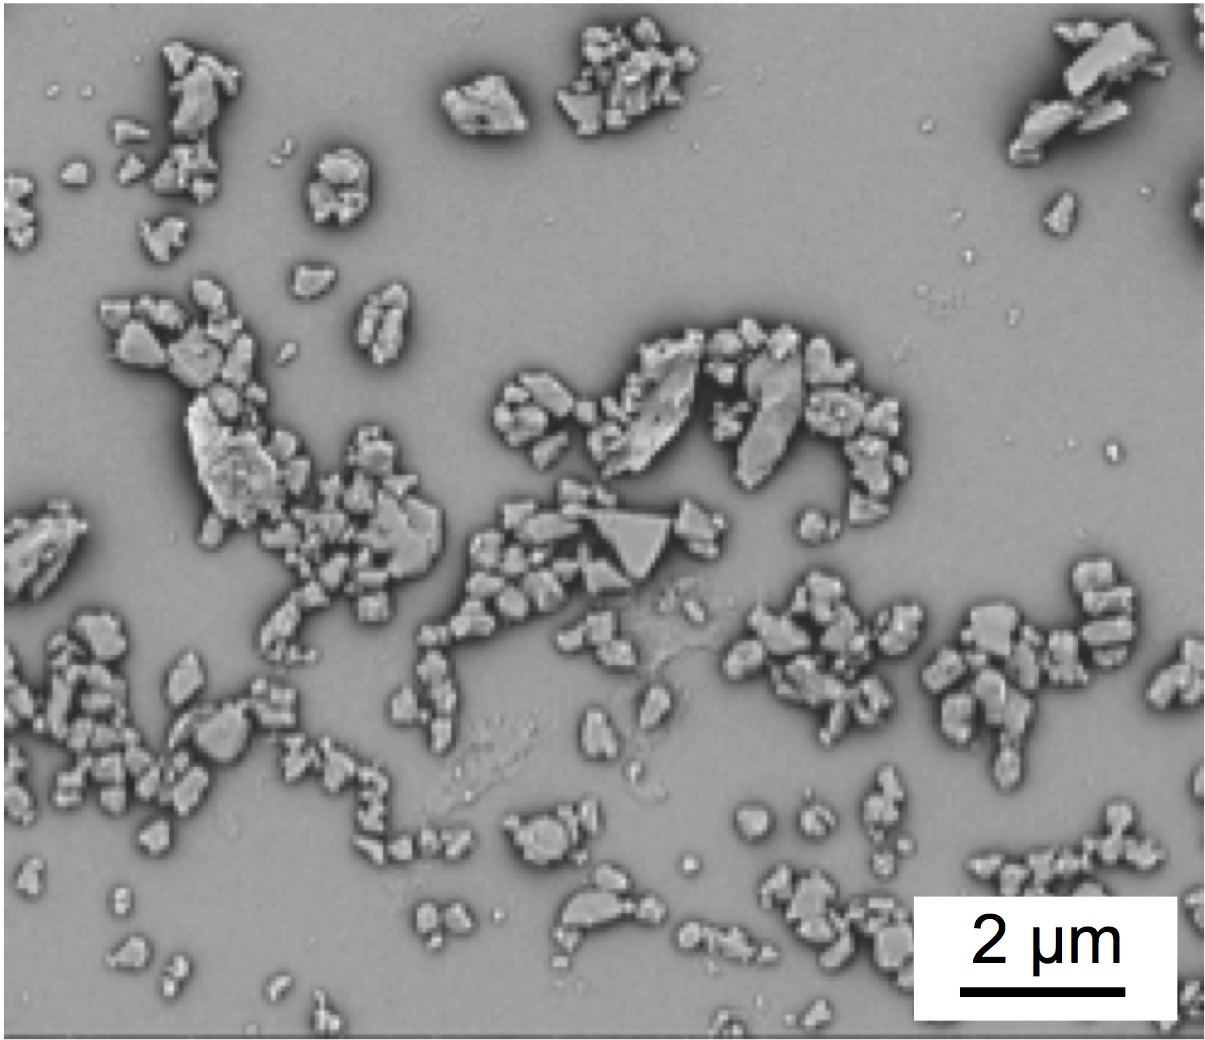
\includegraphics[width=\textwidth]{Chapter-3/Figures/Figure1.png}
	\caption{SEM image of as-received chemically purified Bayer Al$_{2}$O$_{3}$ powder used in this study.}
	\label{Ch3-figure:Figure1}
\end{figure}
%%%

\newpage
%%%
\begin{figure}[H]
	\centering
	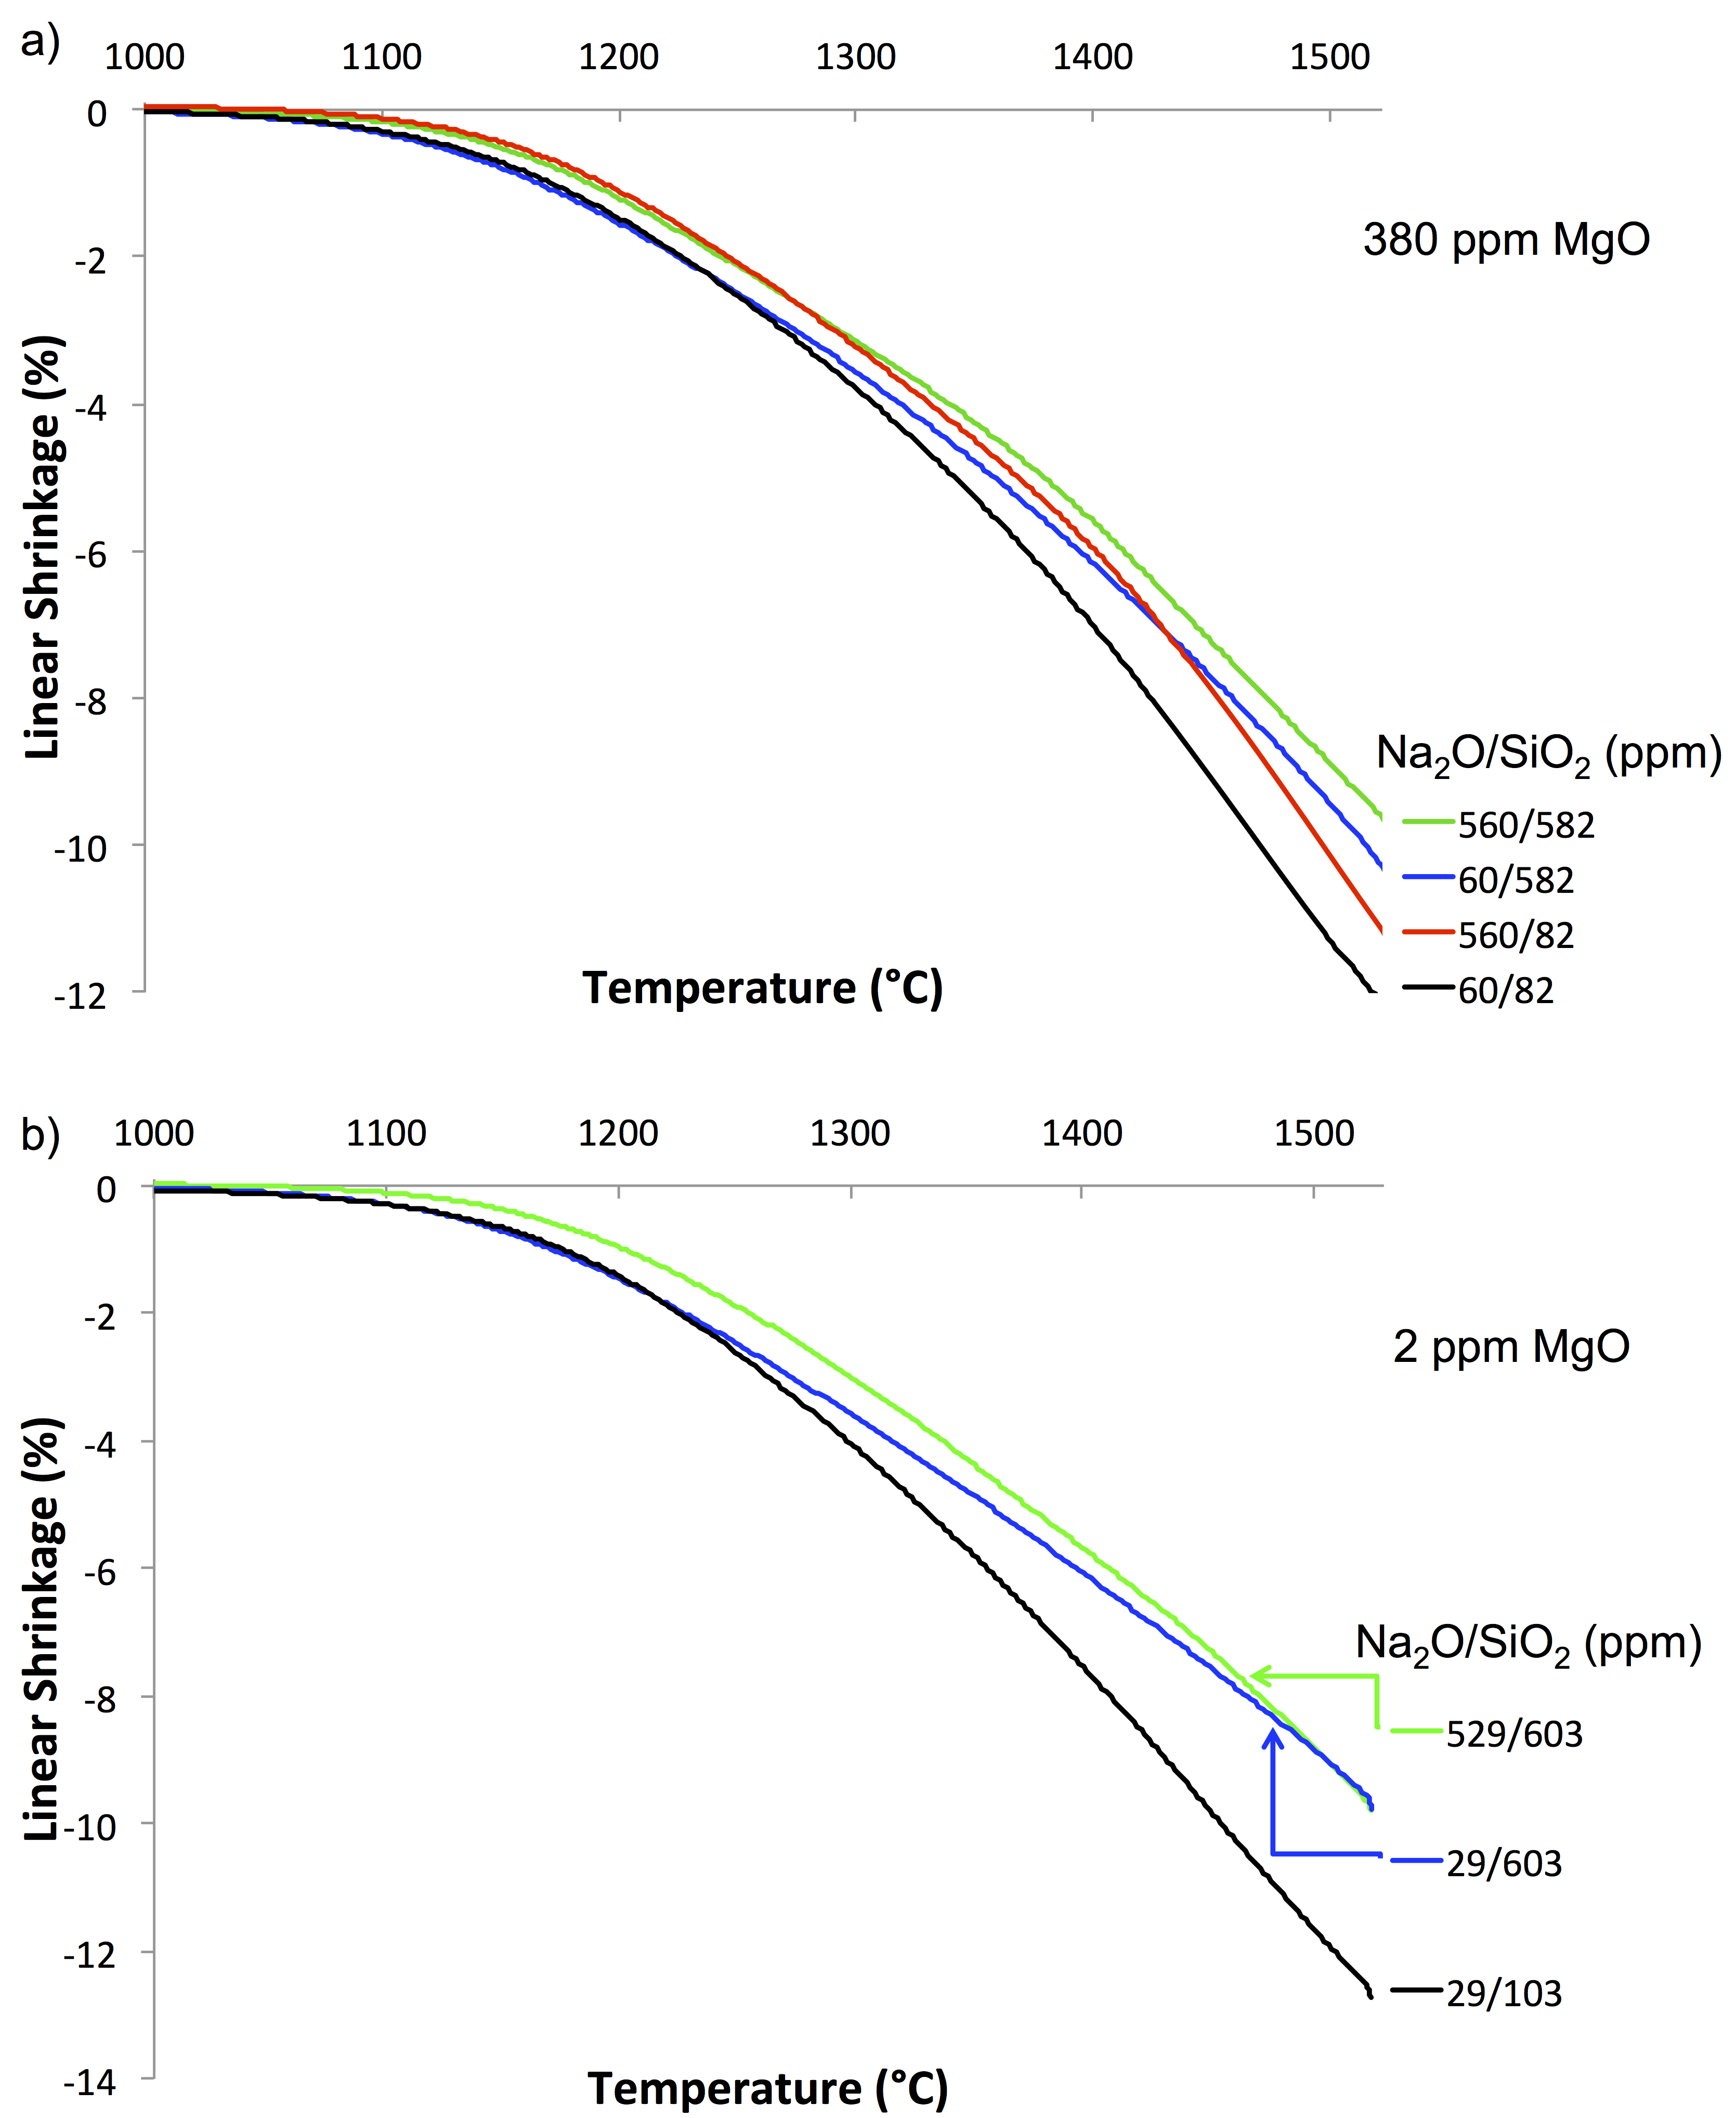
\includegraphics[width=\textwidth]{Chapter-3/Figures/Figure2.png}
	\caption{Dilatometer curves of as-received and singly Na$_{2}$O-doped samples heated at 10$^{\circ}$C/min to 1525$^{\circ}$C.}
	\label{Ch3-figure:Figure2}
\end{figure}
%%%

\newpage
%%%
\begin{figure}[H]
	\centering
	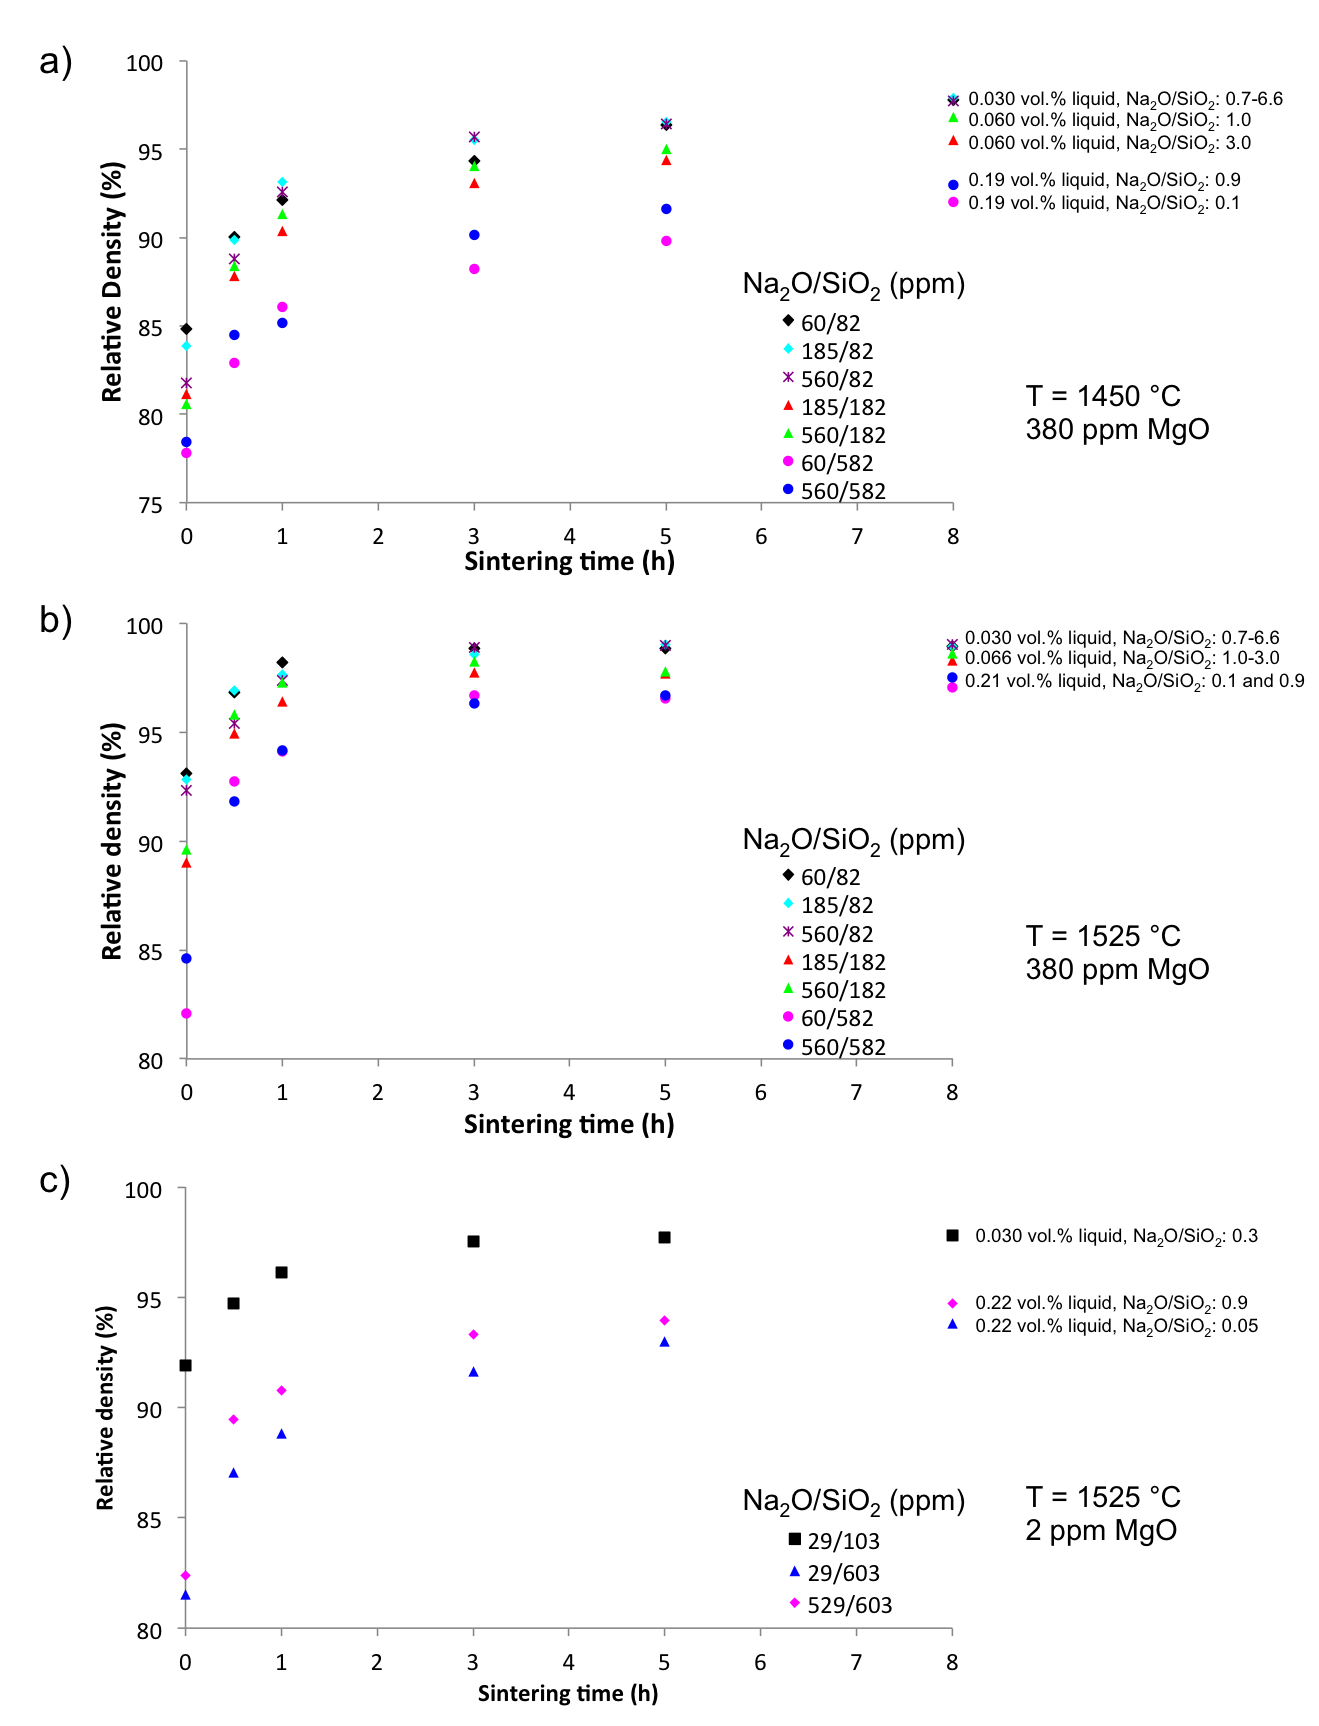
\includegraphics[width=\textwidth]{Chapter-3/Figures/Figure3.png}
	\caption{Densification kinetics of Bayer Al$_{2}$O$_{3}$ doped with different Na$_{2}$O concentrations and sintered at 1525$^{\circ}$C.}
	\label{Ch3-figure:Figure3}
\end{figure}
%%%

\newpage
%%%
\begin{figure}[H]
	\centering
	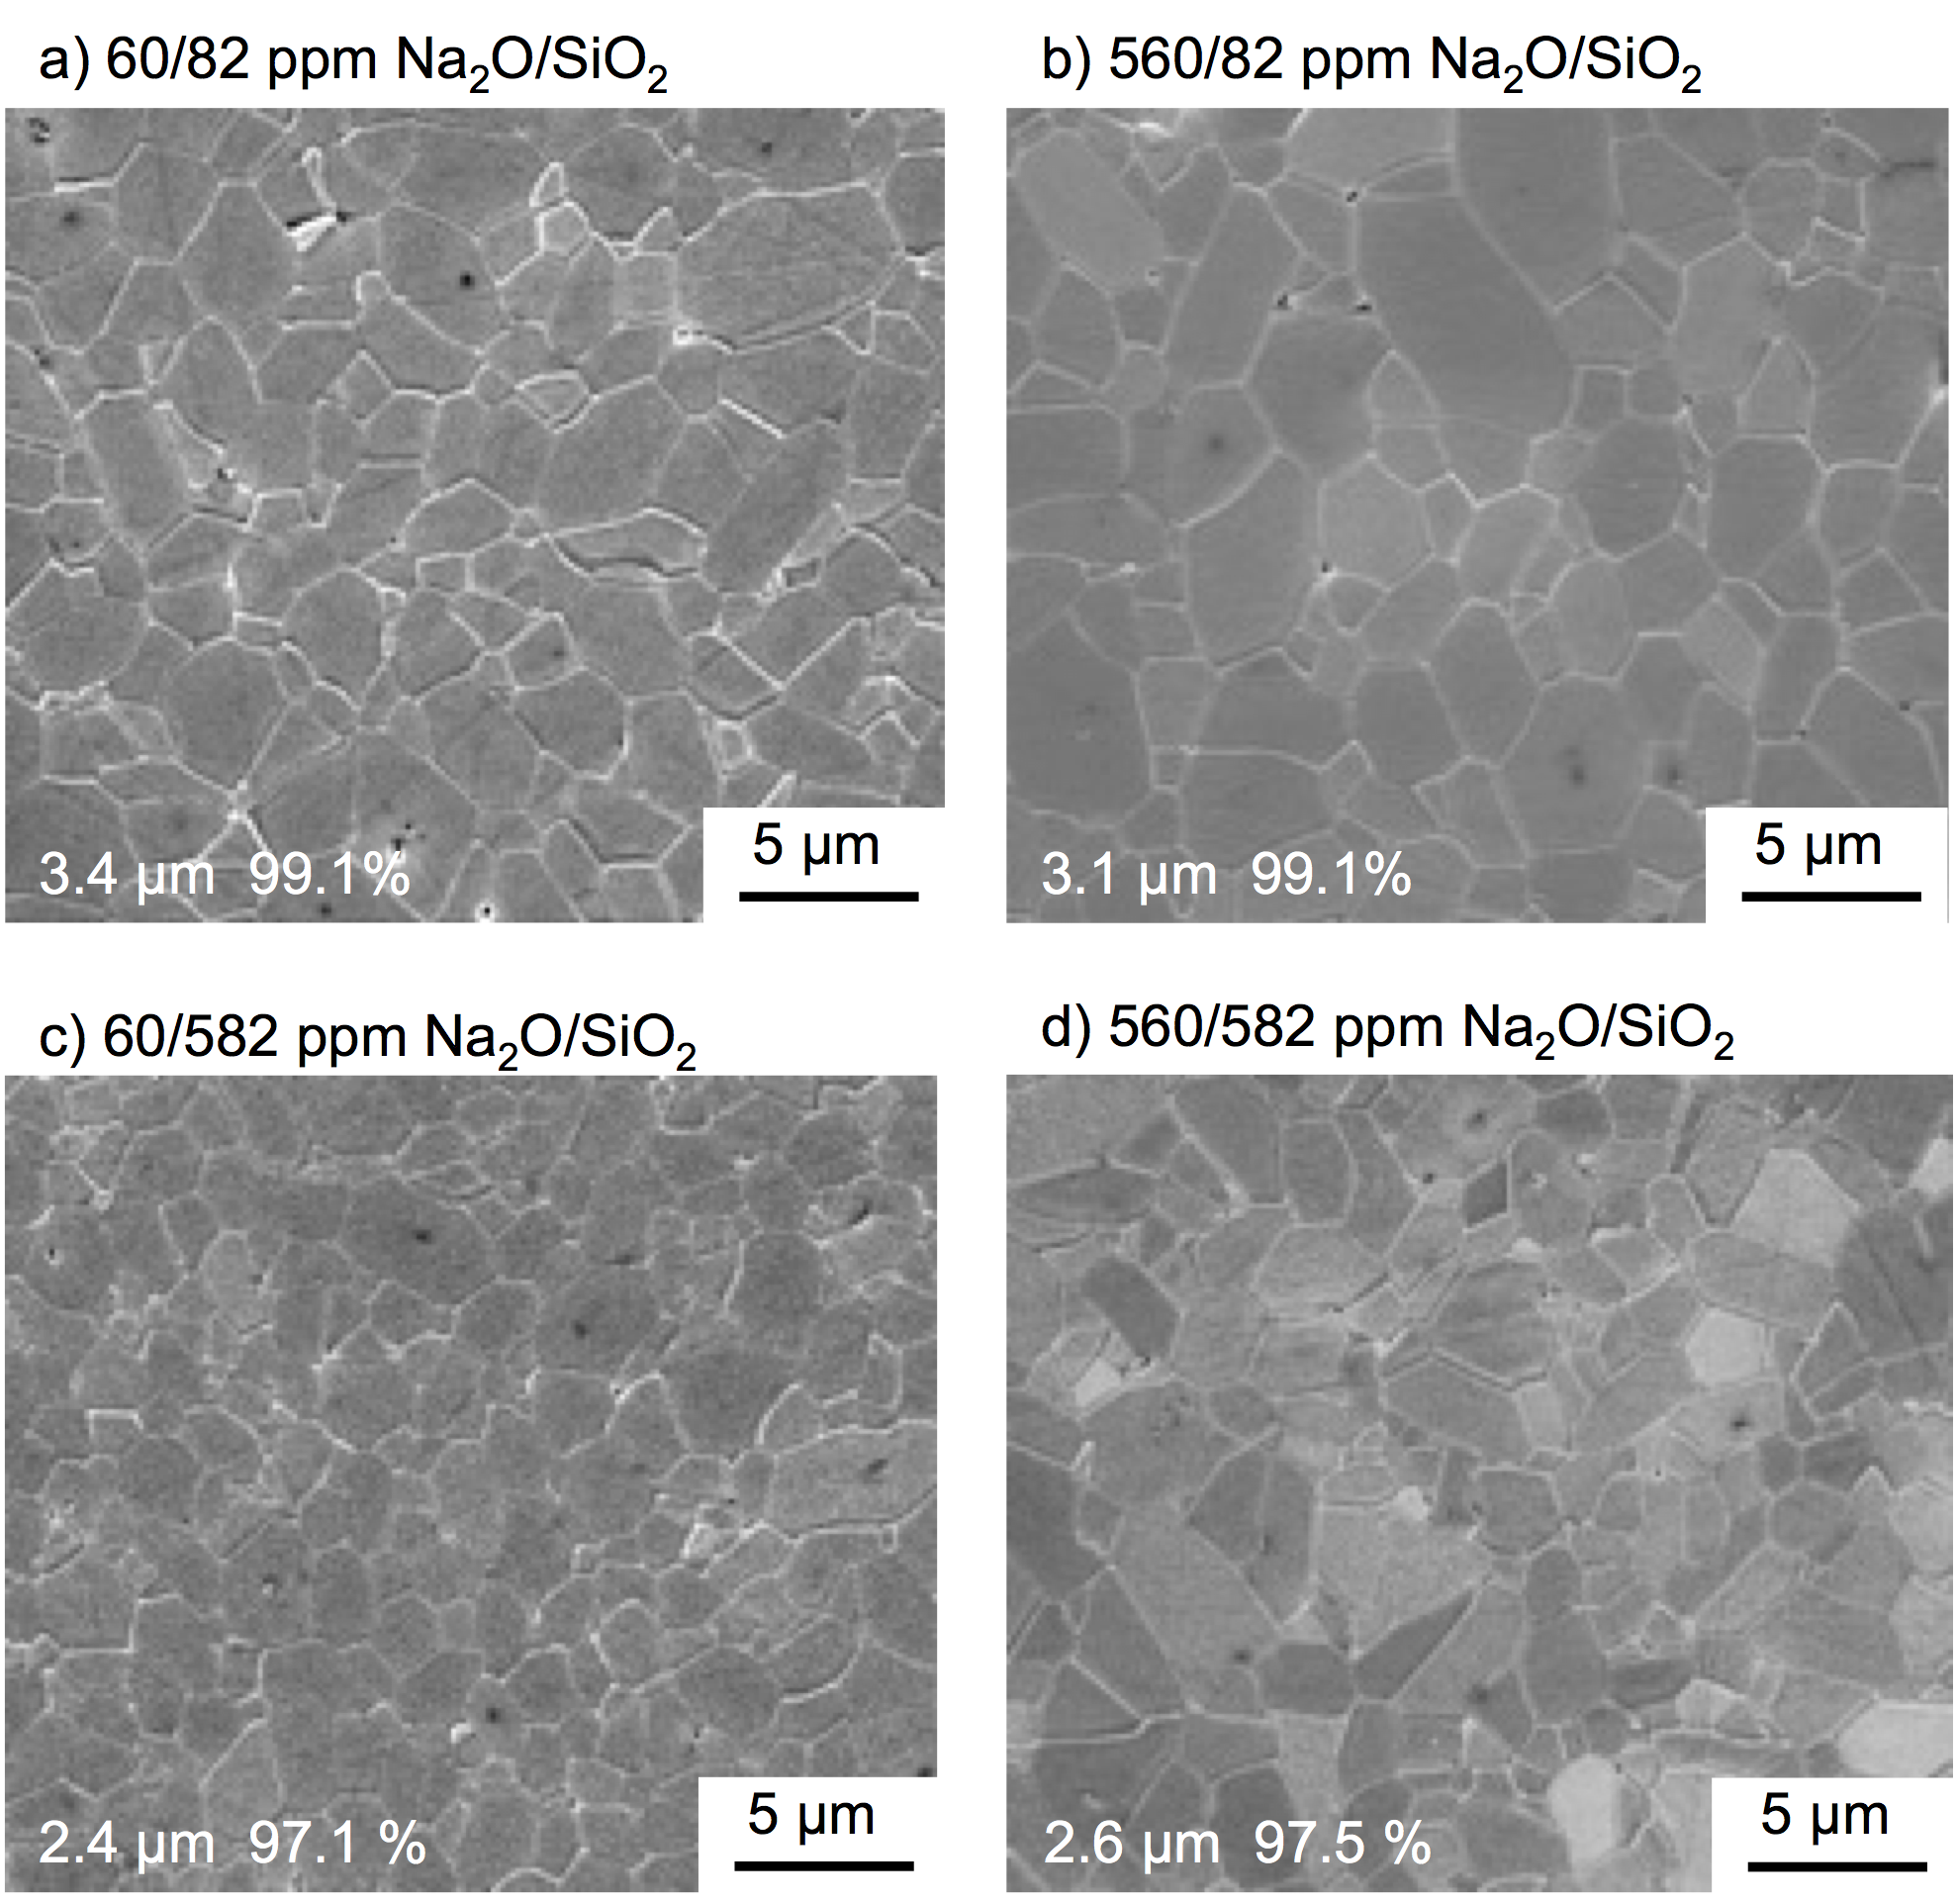
\includegraphics[width=\textwidth]{Chapter-3/Figures/Figure4.png}
	\caption{Microstructures of as-received and singly 529 ppm Na$_{2}$O doped samples after 30 min, 3 h and 8 h at 1525$^{\circ}$C.}
	\label{Ch3-figure:Figure4}
\end{figure}
%%%

\newpage
%%%
\begin{figure}[H]
	\centering
	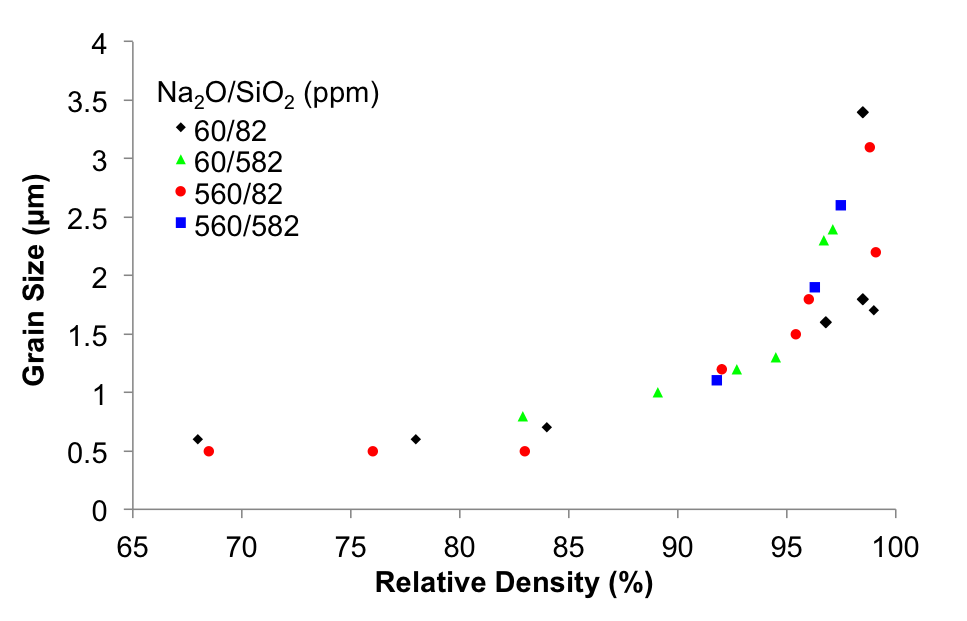
\includegraphics[width=\textwidth]{Chapter-3/Figures/Figure5.png}
	\caption{Dilatometer curves of as-received, singly SiO$_{2}$-doped, and Na$_{2}$O/SiO$_{2}$-doped Bayer Al$_{2}$O$_{3}$ heated at 10$^{\circ}$C/min to 1525$^{\circ}$C.}
	\label{Ch3-figure:Figure5}
\end{figure}
%%%

\newpage
%%%
\begin{figure}[H]
	\centering
	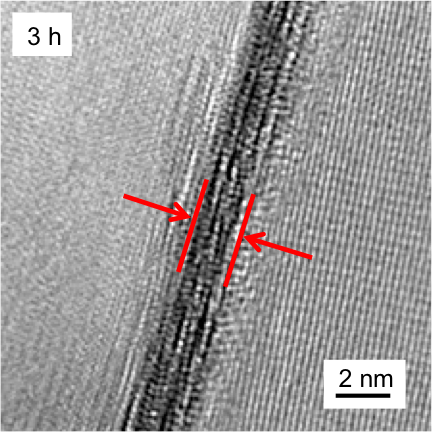
\includegraphics[width=\textwidth]{Chapter-3/Figures/Figure6.png}
	\caption{Densification kinetics of Bayer Al$_{2}$O$_{3}$ doped with different concentrations of Na$_{2}$O and SiO$_{2}$ at 1525$^{\circ}$C.}
	\label{Ch3-figure:Figure6}
\end{figure}
%%%

\newpage
%%%
\begin{figure}[H]
	\centering
	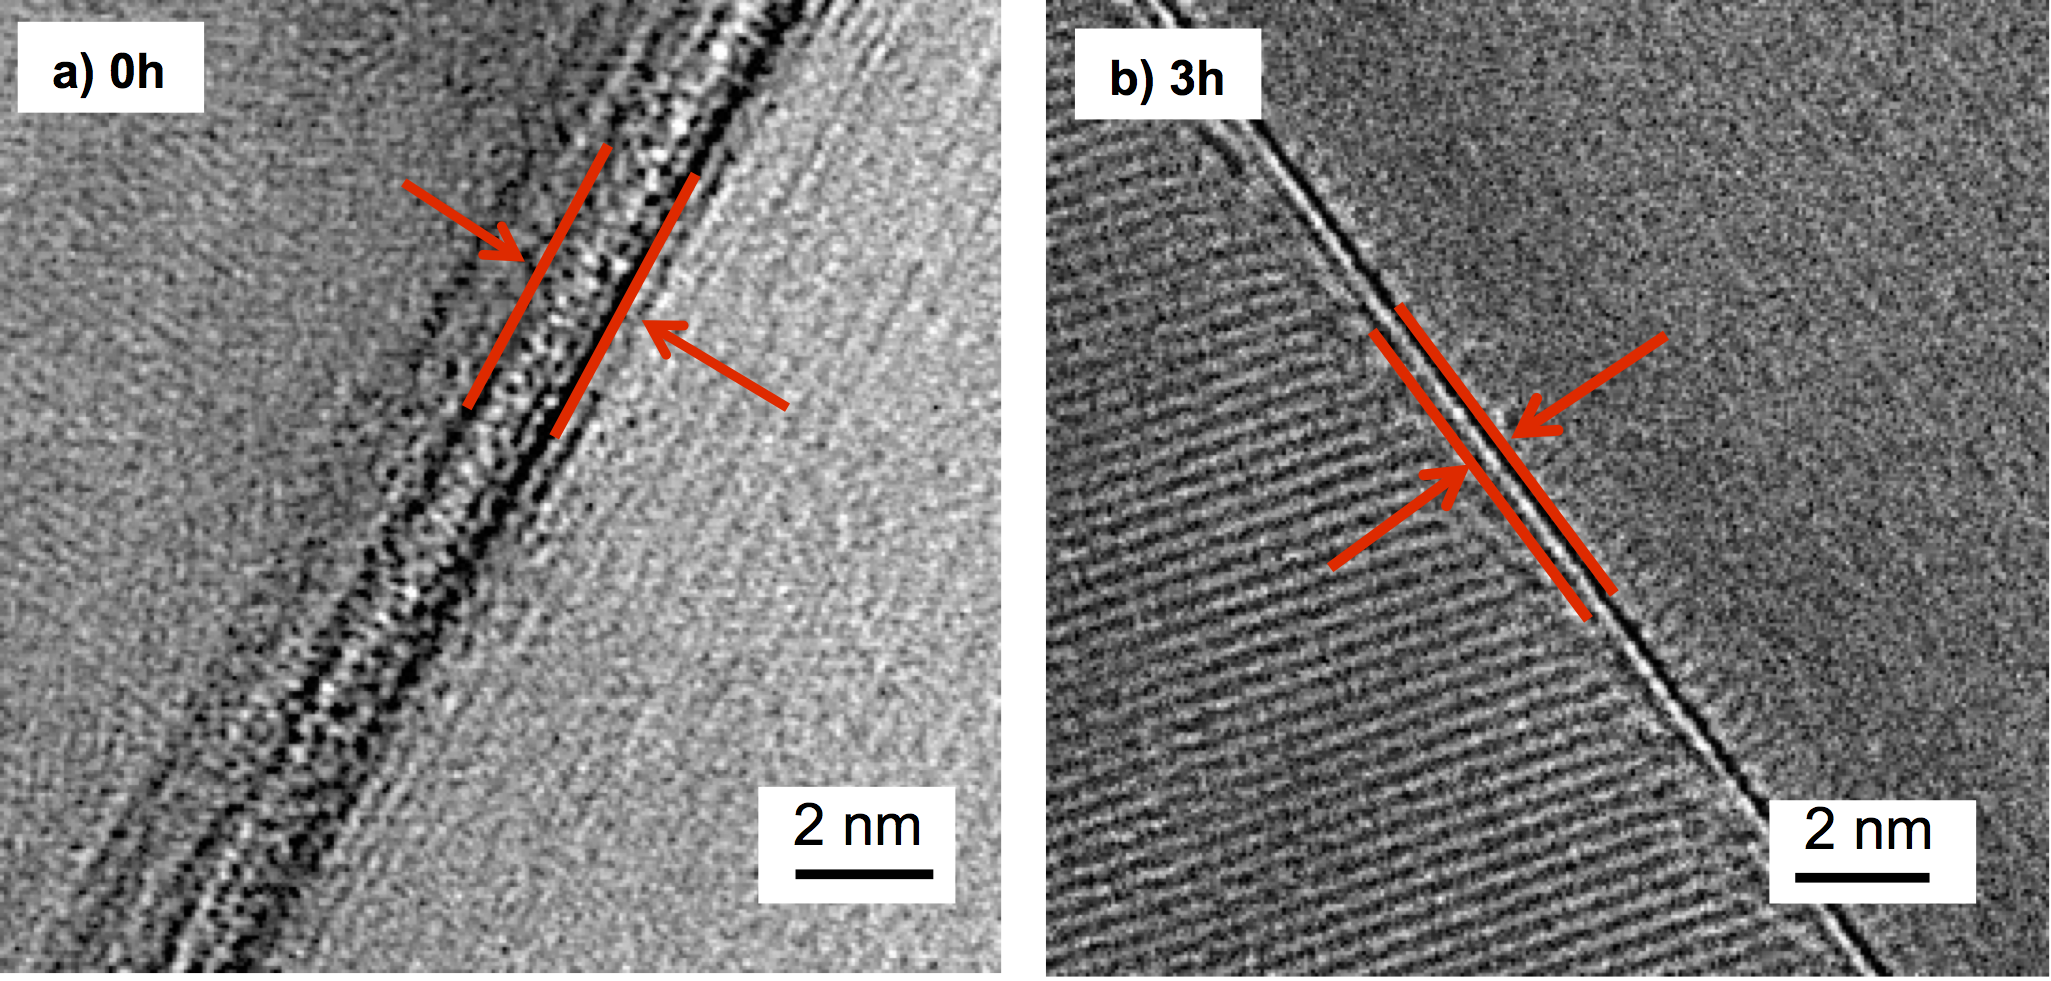
\includegraphics[width=\textwidth]{Chapter-3/Figures/Figure7.png}
	\caption{Microstructures of Bayer Al$_{2}$O$_{3}$ doped with a) 603 ppm SiO$_{2}$ and b) 529 ppm Na$_{2}$O and 603 ppm SiO$_{2}$ after heating at 1525$^{\circ}$C for 8h.}
	\label{Ch3-figure:Figure7}
\end{figure}
%%%

\newpage
%%%
\begin{figure}[H]
	\centering
	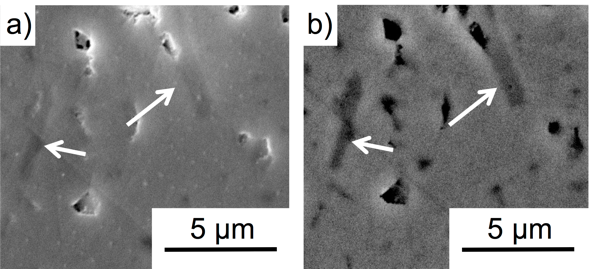
\includegraphics[width=\textwidth]{Chapter-3/Figures/Figure8.png}
	\caption{Micrographs of a sample doped with 1029 ppm Na$_{2}$O after sintering at 1525$^{\circ}$C for 3 h. The micrographs were recorded using a) a secondary electron detector and b) a backscattered electron detector. The arrows point at the platelet shaped beta alumina grains that form in samples doped with Na$_{2}$O. The samples were not thermally etched.}
	\label{Ch3-figure:Figure8}
\end{figure}
%%%

\newpage
%%%
\begin{figure}[H]
	\centering
	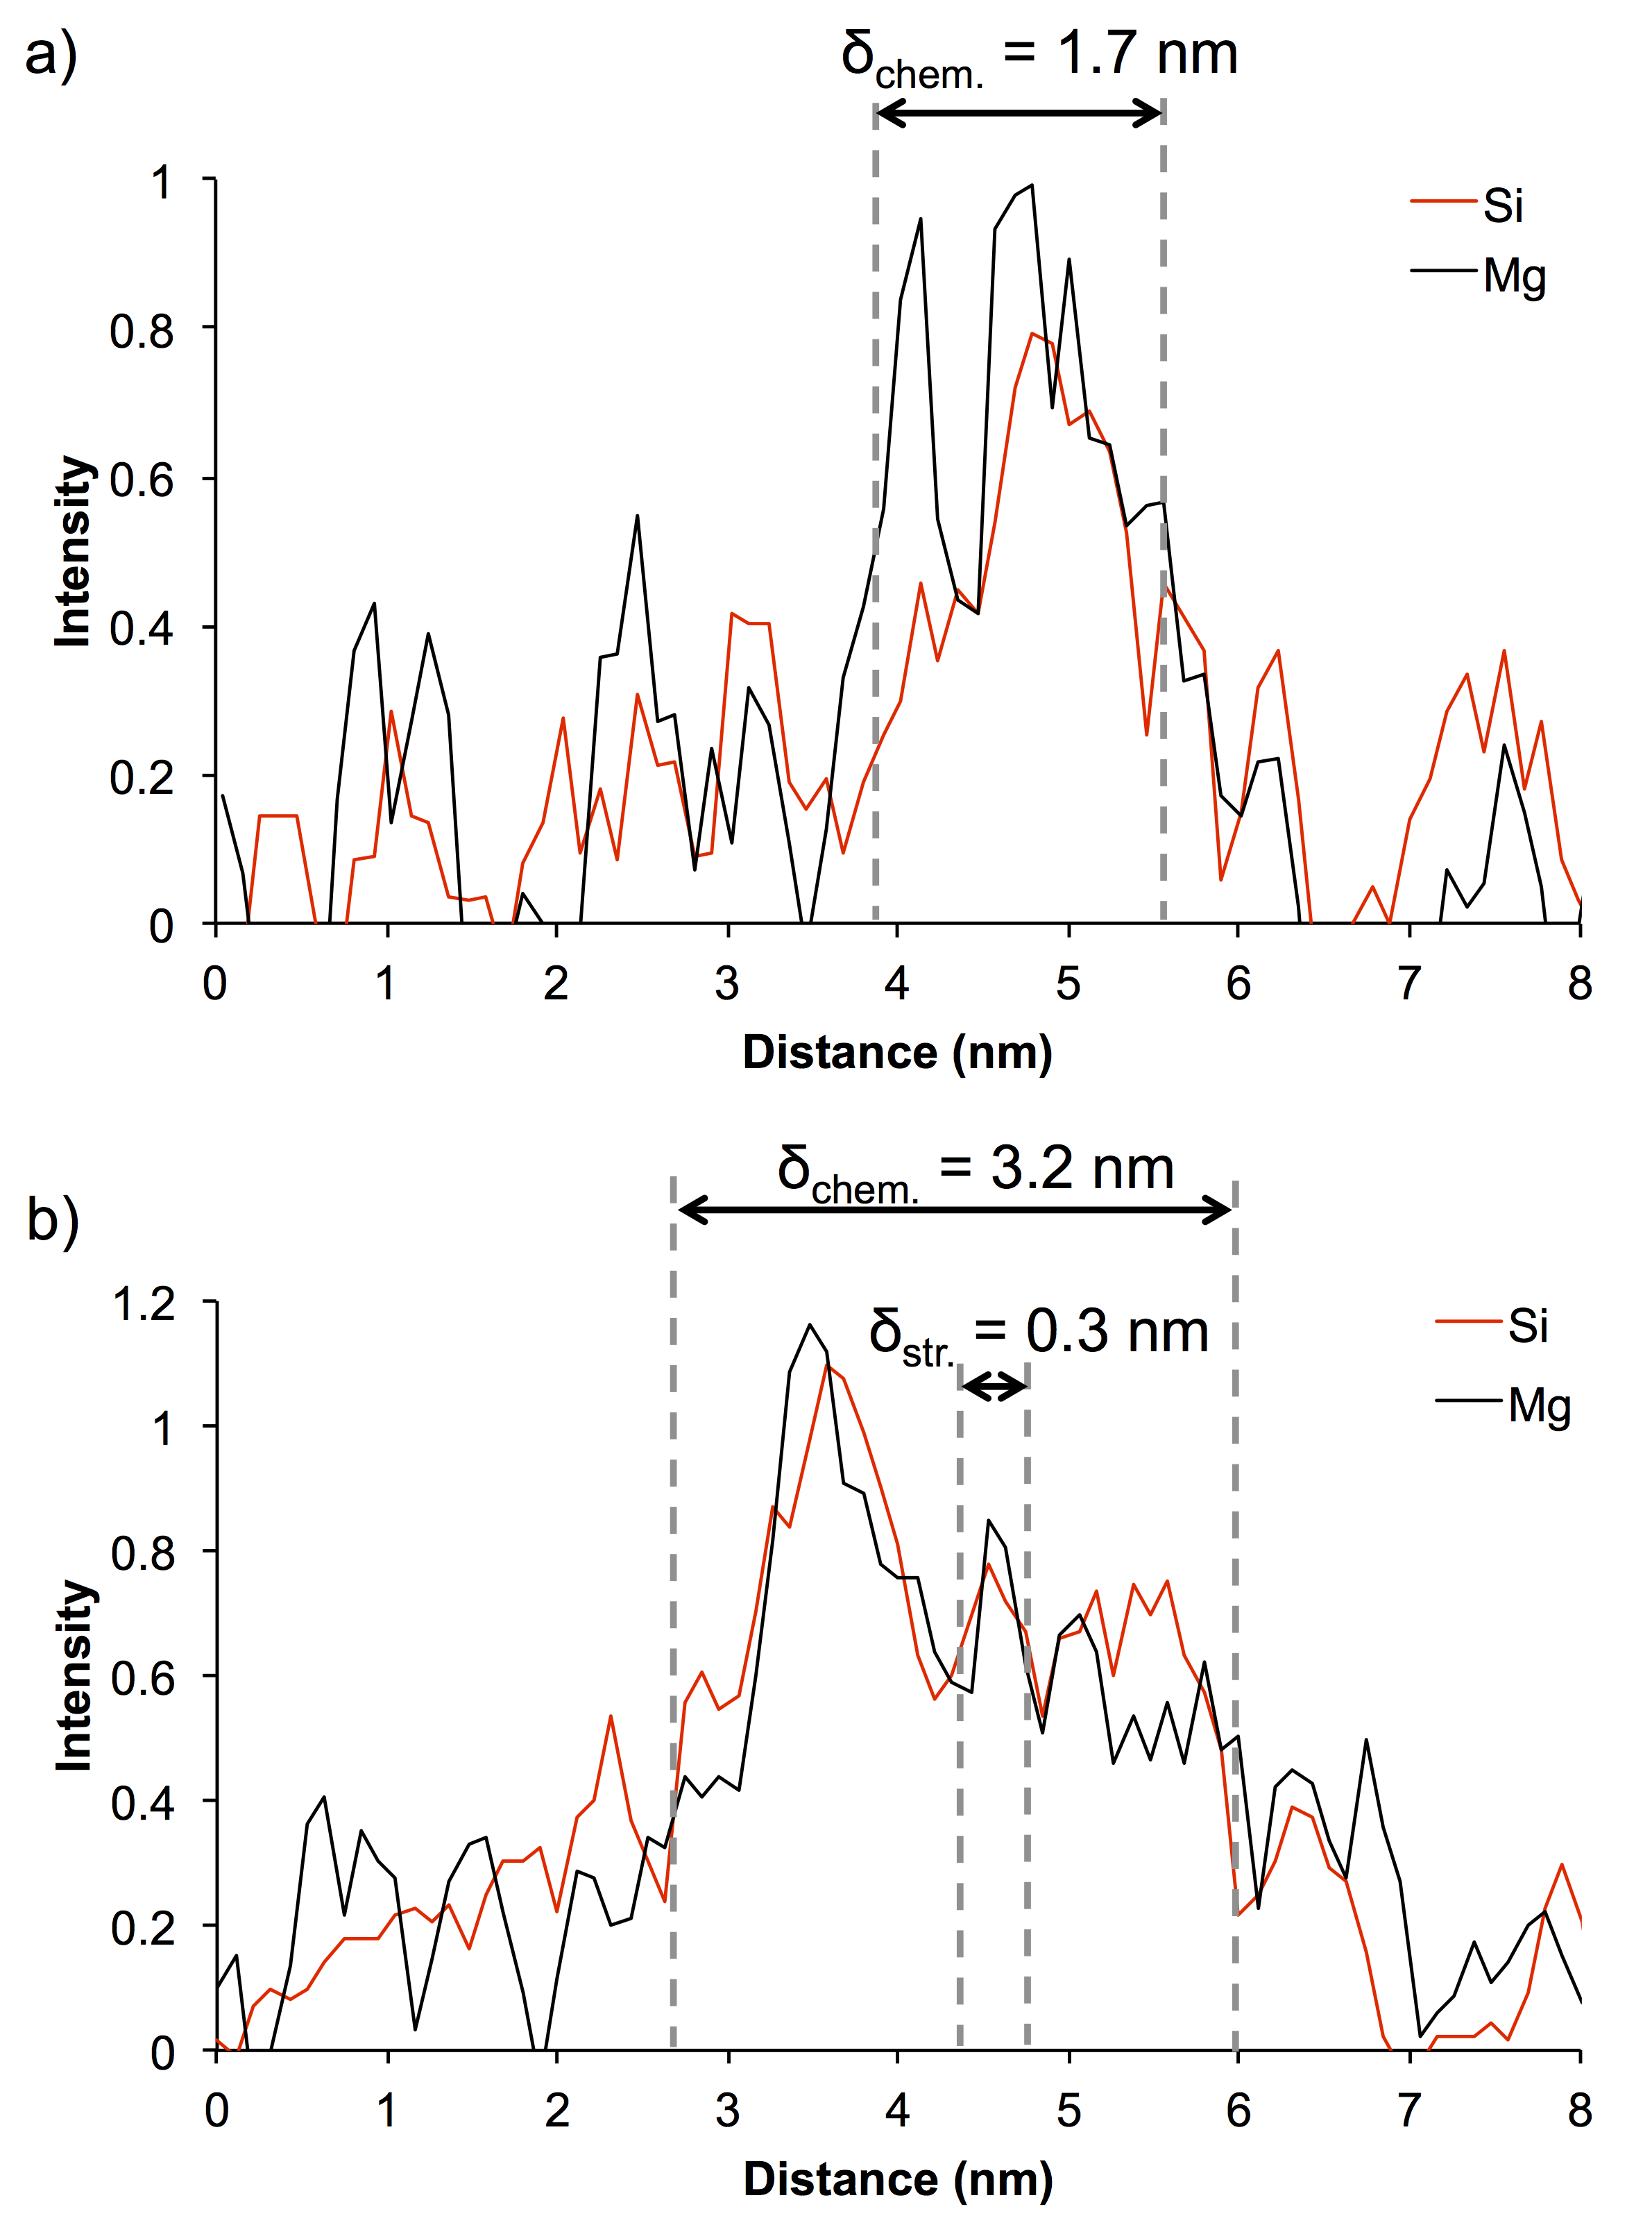
\includegraphics[width=\textwidth]{Chapter-3/Figures/Figure9.png}
	\caption{Liquidus projection of the Al$_{2}$O$_{3}$-SiO$_{2}$-Na$_{2}$O ternary phase diagram. The red solid lines are isoplethal cuts representing the samples investigated in this study. The red dashed line is the 1525$^{\circ}$C isotherm where $\alpha$-Al$_{2}$O$_{3}$ and liquid are in equilibrium. The blue dash-dot line and green dotted line are eutectic lines at which $\alpha$-Al$_{2}$O$_{3}$ and liquid is in equilibrium with $\beta$-Al$_{2}$O$_{3}$ or mullite, respectively.}
	\label{Ch3-figure:Figure9}
\end{figure}
%%%
